The first thing to do is check whether the correlation function gives us an
appropriate response with this sampling rate. In order to do this, we plot the
correlation coefficient of a signal and a pure harmonic vs a change in frequency
about the pure harmonic for \(N\) datapoints. 

The code for plotting these graphs in MATLAB is given here: \\
\begin{itemize}
    \item Code for correlation of 2 signals
\begin{lstlisting}
    
function outp = corel(A,B)
 outp = 0;
 normA = 0;
 normB = 0;
 for i = 1:length(A)
     outp = outp+(A(i)*B(i));
     normA = normA+(A(i)^2);
     normB = normB+ (B(i)^2);
 end
 outp = outp/sqrt(normA*normB);
end
\end{lstlisting} 

\item Code for getting graphs
\begin{lstlisting}
    function grp = coreldraw(f1,f2,f3,f4,phi4)
   t = -0.5:0.005:0.5; %Change the step size to get different resolutions
signal = round(7/3*(sin(f1*t) + sin(f2*t) + sin(f3*t) )) ; %This ensures we have a number between \(\pm7\)
df = -200:0.1:200;
   grp = zeros(length(df));

for i = 1:length(df)
signal2 = round(7*sin(((f4+df(i))*t) + phi4 ));
grp(i) = corel(signal,signal2);
end
plot(df,grp)
xlabel('df')
ylabel('Correlation Coefficient')
s = strcat('Graph of correlation of' ,int2str(f1),'Hz ',int2str(f2),' Hz' ,int2str(f3), ' Hz with ',int2str(f4),' Hz vs change in ',int2str(f4));
title(s)
end
\end{lstlisting}
If we first try correlating with 100 data points, we get 
\begin{figure}[ht]
    \centering
    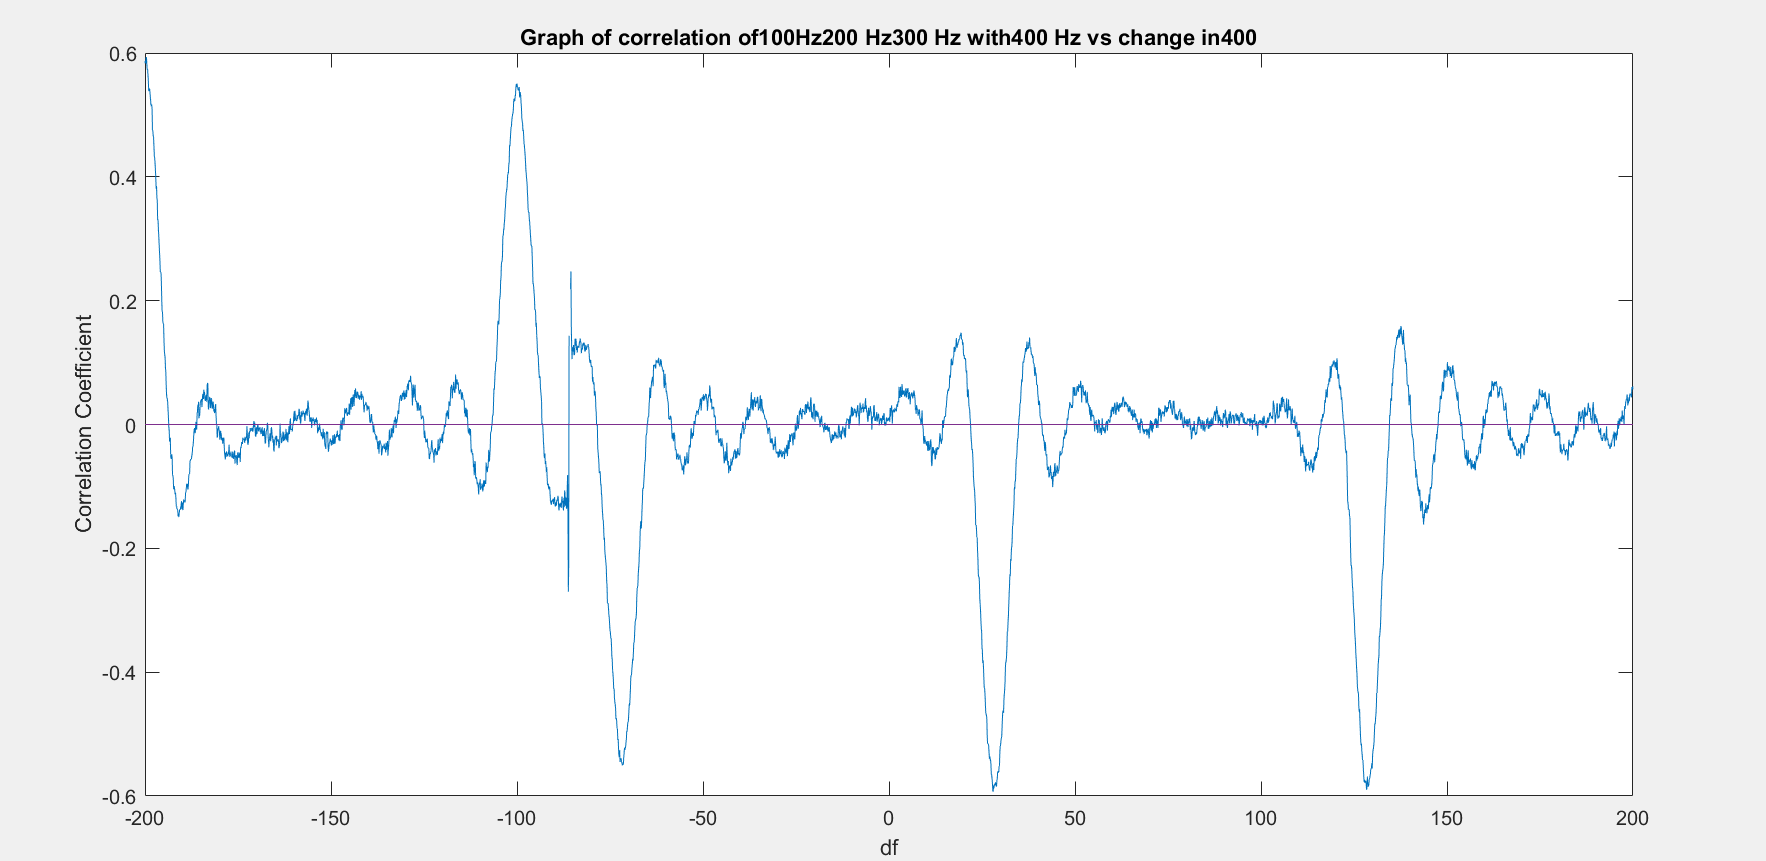
\includegraphics[width=0.6\textwidth]{fig/Graph2100pts.PNG}
    \caption{Correlation with 100 point sampling}
    \label{fig:100pts}
\end{figure}
Clearly, this does not provide a good enough degree of correlation as there are
several significant analolous peaks. We would expect only 2 significant peaks
correspoinding to 200 and 300 Hz. Next we try with 200 points. 
\begin{figure}[ht]
    \centering
    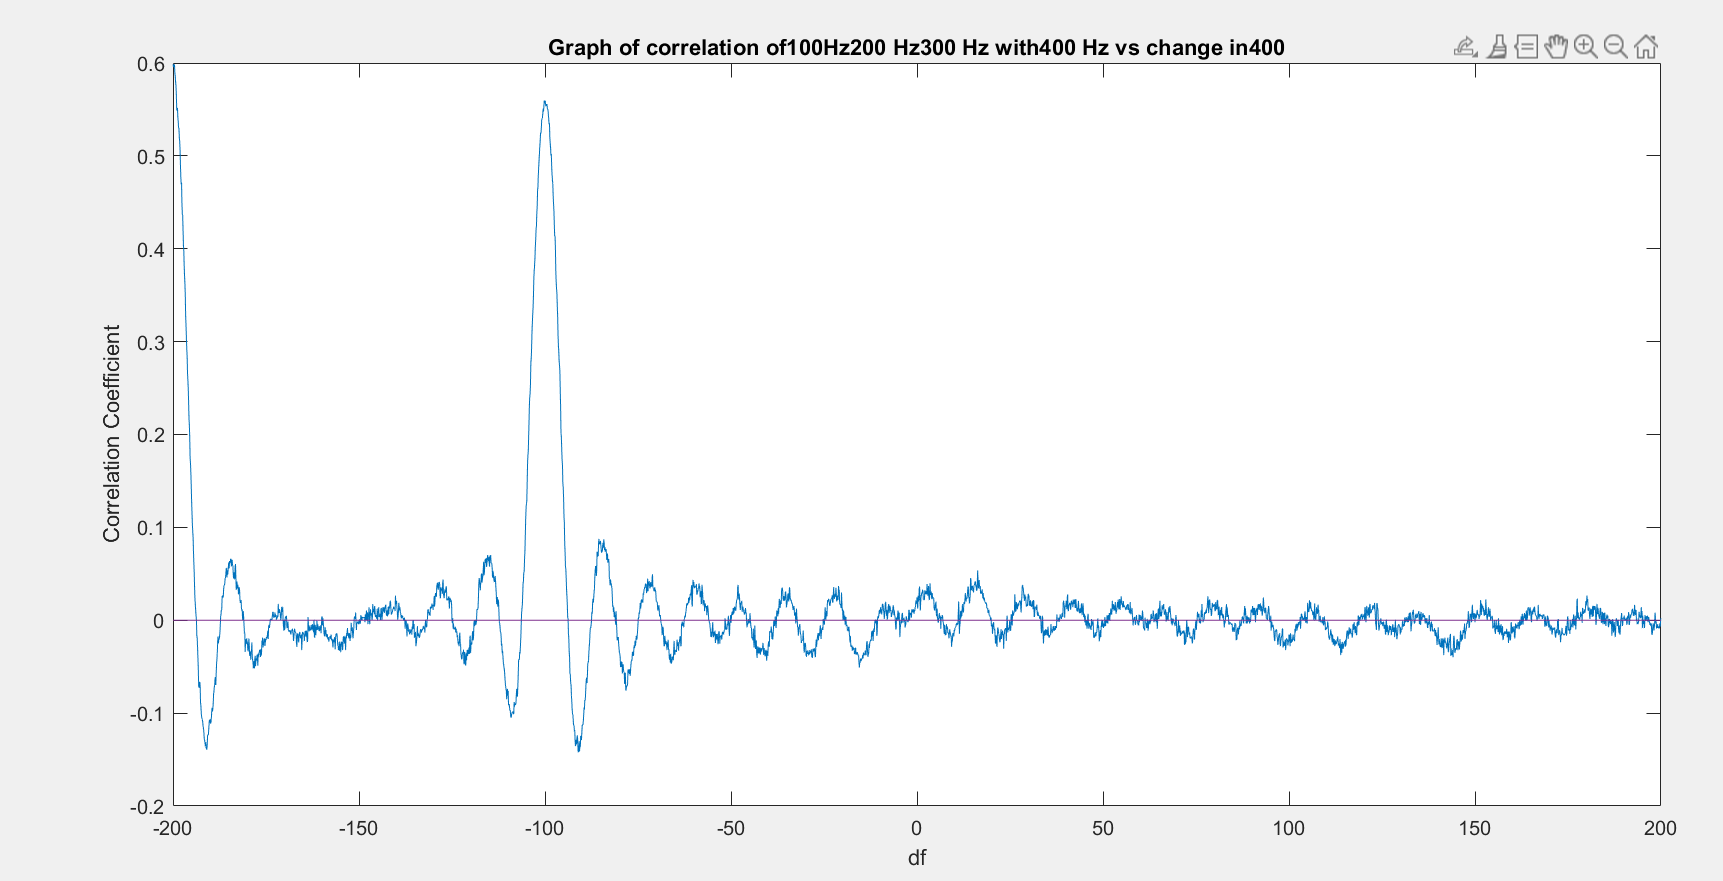
\includegraphics[width=0.6\textwidth]{fig/Graph1.PNG}
    \caption{Correlation with 200 point sampling}
    \label{fig:100pts}
\end{figure}
This gives us very clear peaks at the right frequencies. It appears that 200
points sampling is good enough. In order to check the resolution limit, we also
try a signal where the frequencies are close: 
\begin{figure}[ht]
    \centering
    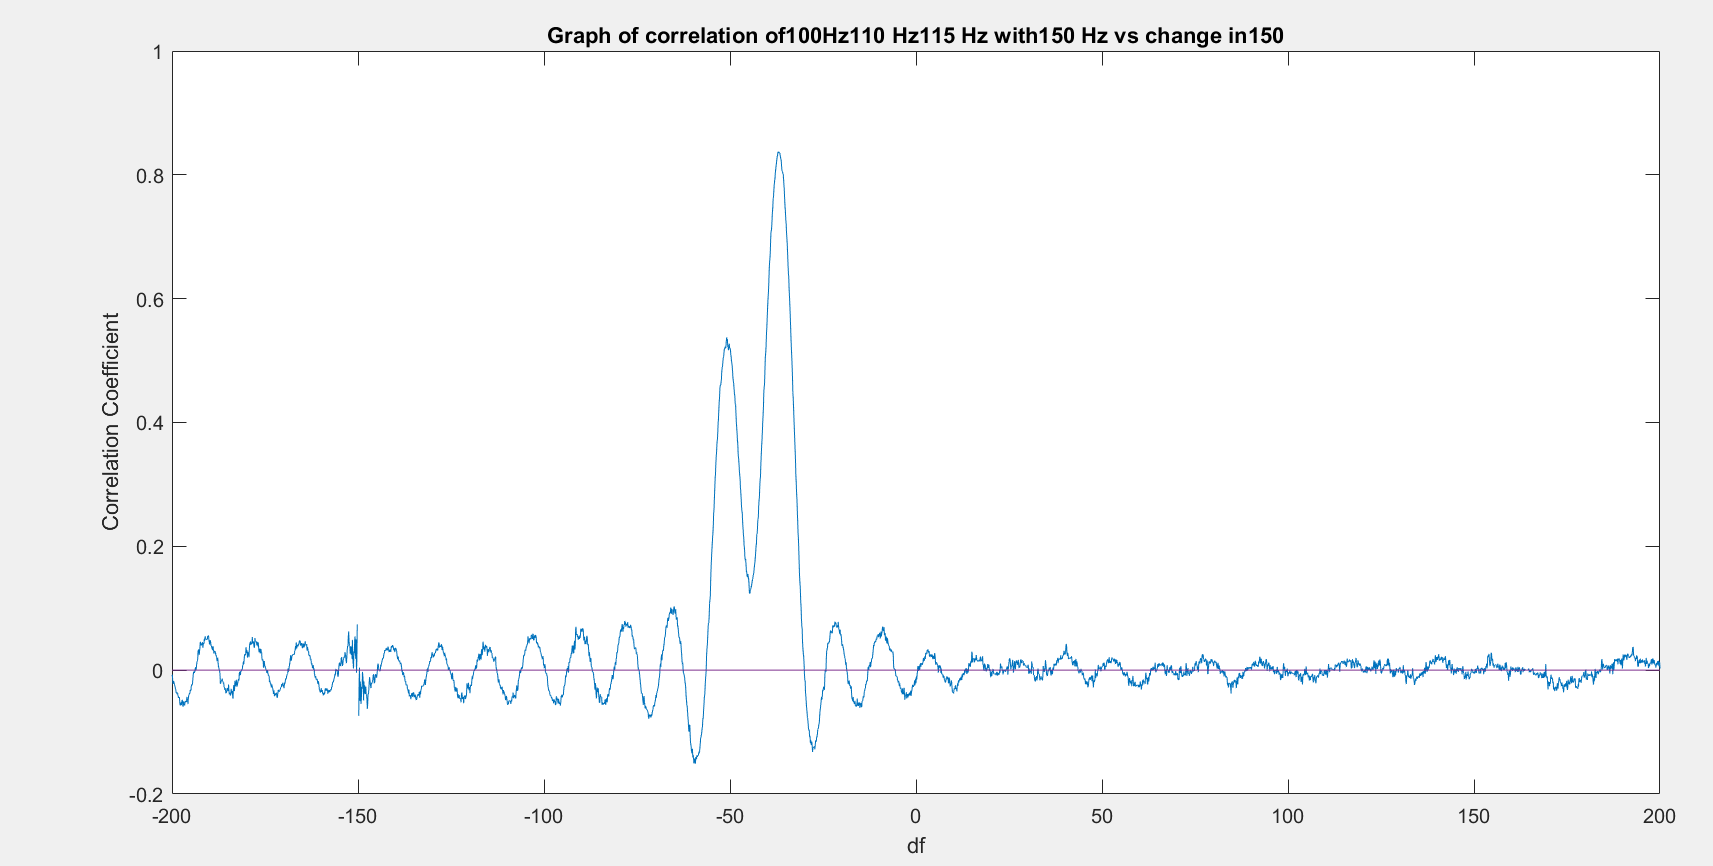
\includegraphics[width=0.6\textwidth]{fig/LowResolutionGraph3200ots.PNG}
    \caption{Correlation with 200 point sampling for 5Hz difference}
    \label{fig:200ptslowres}
\end{figure}
The 3 peaks expected are missed. This implies that we cannot separate
frequencies very close to each other, and this is the price we have to pay for
avoiding a FFT. From these graphs it is clear that a threshold greater than 0.1
will suffice for testing our audio signals. 

\end{itemize}